\documentclass[10pt]{article}
\usepackage{graphicx,fancyhdr,amsmath,amssymb,amsthm,subfig,url,hyperref}
\usepackage[margin=1in]{geometry}
\usepackage{diagbox}
\usepackage{tikz}
%----------------------- Macros and Definitions --------------------------

%%% FILL THIS OUT
%\newcommand{\studentname}{Pramesh Kumar}
%\newcommand{\suid}{kumar372}
\newcommand{\exerciseset}{Homework 4}
%%% END



\renewcommand{\theenumi}{\bf \Alph{enumi}}

%\theoremstyle{plain}
%\newtheorem{theorem}{Theorem}
%\newtheorem{lemma}[theorem]{Lemma}

\fancypagestyle{plain}{}
\pagestyle{fancy}
\fancyhf{}
\fancyhead[RO,LE]{\sffamily\bfseries\large University of Minnesota}
\fancyhead[LO,RE]{\sffamily\bfseries\large CEGE 4011/5214: Transportation Systems Analysis}
%\fancyfoot[LO,RE]{\sffamily\bfseries\large \studentname: \suid @umn.edu}
\fancyfoot[RO,LE]{\sffamily\bfseries\thepage}
\renewcommand{\headrulewidth}{1pt}
\renewcommand{\footrulewidth}{1pt}

\graphicspath{{figures/}}

%-------------------------------- Title ----------------------------------

\title{CEGE 4011/5214 \exerciseset}
%\author{\studentname \qquad x500: \suid}
\date{Due Date: Tuesday, October 13, 2020 11:59 PM}
%--------------------------------- Text ----------------------------------

\begin{document}
\maketitle
\section*{Instructions}
\begin{itemize}
	\setlength\itemsep{0em}
	\item The assignment should be typed or neatly handwritten. If you decide to type your solution, you can use any word processor or LaTeX (a template is uploaded on \href{https://github.com/prameshk/UMN-HW-template}{Gihub}). The final version should be submitted as a PDF document. 
	\item The PDF document should contain the solutions and figures/graphs (if any). Submit computer codes as a supplementary file. All the files should be zipped before submission.
	\item The front page of the homework file should have the name, student ID, and x500 of the student.
	\item You are encouraged to collaborate with other students, but you must submit your solutions individually.
	\item If you have any questions related to homework problems, feel free to email me (Pramesh Kumar (\href{mailto:kumar372@umn.edu}{kumar372@umn.edu})). 
\end{itemize}

\section*{Problem 1}
	Solve the following problems for the network given in Figure \ref{1} using both Gurobi and Networkx and compare the results obtained.
	
	\begin{figure}[h!]
		\centering
		
		
		\tikzset{every picture/.style={line width=0.75pt}} %set default line width to 0.75pt        
		
		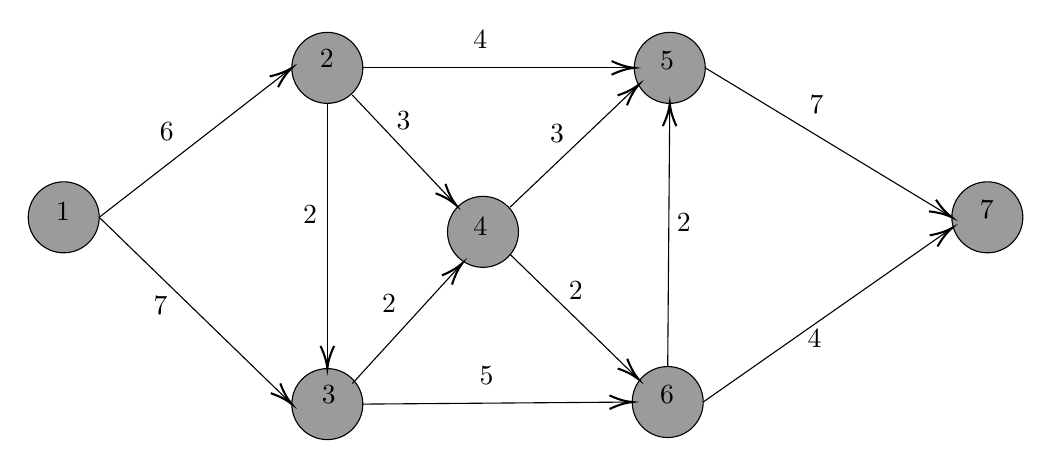
\begin{tikzpicture}[x=0.75pt,y=0.75pt,yscale=-1,xscale=1]
		%uncomment if require: \path (0,300); %set diagram left start at 0, and has height of 300
		
		%Shape: Circle [id:dp7015481174708078] 
		\draw  [fill={rgb, 255:red, 155; green, 155; blue, 155 }  ,fill opacity=1 ] (54.8,138.1) .. controls (54.8,128.66) and (62.46,121) .. (71.9,121) .. controls (81.34,121) and (89,128.66) .. (89,138.1) .. controls (89,147.54) and (81.34,155.2) .. (71.9,155.2) .. controls (62.46,155.2) and (54.8,147.54) .. (54.8,138.1) -- cycle ;
		%Shape: Circle [id:dp7703511656051395] 
		\draw  [fill={rgb, 255:red, 155; green, 155; blue, 155 }  ,fill opacity=1 ] (499.8,138.1) .. controls (499.8,128.66) and (507.46,121) .. (516.9,121) .. controls (526.34,121) and (534,128.66) .. (534,138.1) .. controls (534,147.54) and (526.34,155.2) .. (516.9,155.2) .. controls (507.46,155.2) and (499.8,147.54) .. (499.8,138.1) -- cycle ;
		%Shape: Circle [id:dp7251307972190368] 
		\draw  [fill={rgb, 255:red, 155; green, 155; blue, 155 }  ,fill opacity=1 ] (181.8,66.1) .. controls (181.8,56.66) and (189.46,49) .. (198.9,49) .. controls (208.34,49) and (216,56.66) .. (216,66.1) .. controls (216,75.54) and (208.34,83.2) .. (198.9,83.2) .. controls (189.46,83.2) and (181.8,75.54) .. (181.8,66.1) -- cycle ;
		%Shape: Circle [id:dp7408846415079978] 
		\draw  [fill={rgb, 255:red, 155; green, 155; blue, 155 }  ,fill opacity=1 ] (346.8,66.1) .. controls (346.8,56.66) and (354.46,49) .. (363.9,49) .. controls (373.34,49) and (381,56.66) .. (381,66.1) .. controls (381,75.54) and (373.34,83.2) .. (363.9,83.2) .. controls (354.46,83.2) and (346.8,75.54) .. (346.8,66.1) -- cycle ;
		%Shape: Circle [id:dp41644865023795485] 
		\draw  [fill={rgb, 255:red, 155; green, 155; blue, 155 }  ,fill opacity=1 ] (181.8,228.1) .. controls (181.8,218.66) and (189.46,211) .. (198.9,211) .. controls (208.34,211) and (216,218.66) .. (216,228.1) .. controls (216,237.54) and (208.34,245.2) .. (198.9,245.2) .. controls (189.46,245.2) and (181.8,237.54) .. (181.8,228.1) -- cycle ;
		%Shape: Circle [id:dp19888566401613983] 
		\draw  [fill={rgb, 255:red, 155; green, 155; blue, 155 }  ,fill opacity=1 ] (345.8,227.1) .. controls (345.8,217.66) and (353.46,210) .. (362.9,210) .. controls (372.34,210) and (380,217.66) .. (380,227.1) .. controls (380,236.54) and (372.34,244.2) .. (362.9,244.2) .. controls (353.46,244.2) and (345.8,236.54) .. (345.8,227.1) -- cycle ;
		%Straight Lines [id:da5206700636592757] 
		\draw    (89,138.1) -- (180.22,67.33) ;
		\draw [shift={(181.8,66.1)}, rotate = 502.19] [color={rgb, 255:red, 0; green, 0; blue, 0 }  ][line width=0.75]    (10.93,-3.29) .. controls (6.95,-1.4) and (3.31,-0.3) .. (0,0) .. controls (3.31,0.3) and (6.95,1.4) .. (10.93,3.29)   ;
		%Straight Lines [id:da34503373239565127] 
		\draw    (89,138.1) -- (180.36,226.71) ;
		\draw [shift={(181.8,228.1)}, rotate = 224.12] [color={rgb, 255:red, 0; green, 0; blue, 0 }  ][line width=0.75]    (10.93,-3.29) .. controls (6.95,-1.4) and (3.31,-0.3) .. (0,0) .. controls (3.31,0.3) and (6.95,1.4) .. (10.93,3.29)   ;
		%Straight Lines [id:da5253797261113626] 
		\draw    (198.9,83.2) -- (198.9,209) ;
		\draw [shift={(198.9,211)}, rotate = 270] [color={rgb, 255:red, 0; green, 0; blue, 0 }  ][line width=0.75]    (10.93,-3.29) .. controls (6.95,-1.4) and (3.31,-0.3) .. (0,0) .. controls (3.31,0.3) and (6.95,1.4) .. (10.93,3.29)   ;
		%Straight Lines [id:da9051047252301394] 
		\draw    (216,66.1) -- (344.8,66.1) ;
		\draw [shift={(346.8,66.1)}, rotate = 180] [color={rgb, 255:red, 0; green, 0; blue, 0 }  ][line width=0.75]    (10.93,-3.29) .. controls (6.95,-1.4) and (3.31,-0.3) .. (0,0) .. controls (3.31,0.3) and (6.95,1.4) .. (10.93,3.29)   ;
		%Straight Lines [id:da5687966905274591] 
		\draw    (216,228.1) -- (343.8,227.12) ;
		\draw [shift={(345.8,227.1)}, rotate = 539.56] [color={rgb, 255:red, 0; green, 0; blue, 0 }  ][line width=0.75]    (10.93,-3.29) .. controls (6.95,-1.4) and (3.31,-0.3) .. (0,0) .. controls (3.31,0.3) and (6.95,1.4) .. (10.93,3.29)   ;
		%Shape: Circle [id:dp7177536593962709] 
		\draw  [fill={rgb, 255:red, 155; green, 155; blue, 155 }  ,fill opacity=1 ] (256.8,145.1) .. controls (256.8,135.66) and (264.46,128) .. (273.9,128) .. controls (283.34,128) and (291,135.66) .. (291,145.1) .. controls (291,154.54) and (283.34,162.2) .. (273.9,162.2) .. controls (264.46,162.2) and (256.8,154.54) .. (256.8,145.1) -- cycle ;
		%Straight Lines [id:da5717321689480849] 
		\draw    (210.95,79.2) -- (259.58,130.75) ;
		\draw [shift={(260.95,132.2)}, rotate = 226.67000000000002] [color={rgb, 255:red, 0; green, 0; blue, 0 }  ][line width=0.75]    (10.93,-3.29) .. controls (6.95,-1.4) and (3.31,-0.3) .. (0,0) .. controls (3.31,0.3) and (6.95,1.4) .. (10.93,3.29)   ;
		%Straight Lines [id:da41406569785778036] 
		\draw    (287,156) -- (347.52,214.81) ;
		\draw [shift={(348.95,216.2)}, rotate = 224.18] [color={rgb, 255:red, 0; green, 0; blue, 0 }  ][line width=0.75]    (10.93,-3.29) .. controls (6.95,-1.4) and (3.31,-0.3) .. (0,0) .. controls (3.31,0.3) and (6.95,1.4) .. (10.93,3.29)   ;
		%Straight Lines [id:da5082366645869035] 
		\draw    (210.95,218.2) -- (262.6,161.68) ;
		\draw [shift={(263.95,160.2)}, rotate = 492.42] [color={rgb, 255:red, 0; green, 0; blue, 0 }  ][line width=0.75]    (10.93,-3.29) .. controls (6.95,-1.4) and (3.31,-0.3) .. (0,0) .. controls (3.31,0.3) and (6.95,1.4) .. (10.93,3.29)   ;
		%Straight Lines [id:da3535173985818423] 
		\draw    (286.95,133.2) -- (347.5,75.58) ;
		\draw [shift={(348.95,74.2)}, rotate = 496.42] [color={rgb, 255:red, 0; green, 0; blue, 0 }  ][line width=0.75]    (10.93,-3.29) .. controls (6.95,-1.4) and (3.31,-0.3) .. (0,0) .. controls (3.31,0.3) and (6.95,1.4) .. (10.93,3.29)   ;
		%Straight Lines [id:da6627172820993644] 
		\draw    (362.9,210) -- (363.88,85.2) ;
		\draw [shift={(363.9,83.2)}, rotate = 450.45] [color={rgb, 255:red, 0; green, 0; blue, 0 }  ][line width=0.75]    (10.93,-3.29) .. controls (6.95,-1.4) and (3.31,-0.3) .. (0,0) .. controls (3.31,0.3) and (6.95,1.4) .. (10.93,3.29)   ;
		%Straight Lines [id:da17632588209314792] 
		\draw    (381,66.1) -- (498.09,137.06) ;
		\draw [shift={(499.8,138.1)}, rotate = 211.22] [color={rgb, 255:red, 0; green, 0; blue, 0 }  ][line width=0.75]    (10.93,-3.29) .. controls (6.95,-1.4) and (3.31,-0.3) .. (0,0) .. controls (3.31,0.3) and (6.95,1.4) .. (10.93,3.29)   ;
		%Straight Lines [id:da5723812731146496] 
		\draw    (380,227.1) -- (498.31,144.35) ;
		\draw [shift={(499.95,143.2)}, rotate = 505.03] [color={rgb, 255:red, 0; green, 0; blue, 0 }  ][line width=0.75]    (10.93,-3.29) .. controls (6.95,-1.4) and (3.31,-0.3) .. (0,0) .. controls (3.31,0.3) and (6.95,1.4) .. (10.93,3.29)   ;
		
		% Text Node
		\draw (122,138) node [anchor=north west][inner sep=0.75pt]   [align=left] {$ $};
		% Text Node
		\draw (117,91) node [anchor=north west][inner sep=0.75pt]   [align=left] {$\displaystyle 6$};
		% Text Node
		\draw (114,175) node [anchor=north west][inner sep=0.75pt]   [align=left] {$\displaystyle 7$};
		% Text Node
		\draw (268,47) node [anchor=north west][inner sep=0.75pt]   [align=left] {$\displaystyle 4$};
		% Text Node
		\draw (231,86) node [anchor=north west][inner sep=0.75pt]   [align=left] {$\displaystyle 3$};
		% Text Node
		\draw (305,92) node [anchor=north west][inner sep=0.75pt]   [align=left] {3};
		% Text Node
		\draw (224,174) node [anchor=north west][inner sep=0.75pt]   [align=left] {2};
		% Text Node
		\draw (314,168) node [anchor=north west][inner sep=0.75pt]   [align=left] {$\displaystyle 2$};
		% Text Node
		\draw (271,209) node [anchor=north west][inner sep=0.75pt]   [align=left] {$\displaystyle 5$};
		% Text Node
		\draw (366,135) node [anchor=north west][inner sep=0.75pt]   [align=left] {$\displaystyle 2$};
		% Text Node
		\draw (430,78) node [anchor=north west][inner sep=0.75pt]   [align=left] {$\displaystyle 7$};
		% Text Node
		\draw (429,191) node [anchor=north west][inner sep=0.75pt]   [align=left] {$\displaystyle 4$};
		% Text Node
		\draw (67,130) node [anchor=north west][inner sep=0.75pt]   [align=left] {$\displaystyle 1$};
		% Text Node
		\draw (194,56) node [anchor=north west][inner sep=0.75pt]   [align=left] {$\displaystyle 2$};
		% Text Node
		\draw (195,218) node [anchor=north west][inner sep=0.75pt]   [align=left] {$\displaystyle 3$};
		% Text Node
		\draw (268,137) node [anchor=north west][inner sep=0.75pt]   [align=left] {$\displaystyle 4$};
		% Text Node
		\draw (358,57) node [anchor=north west][inner sep=0.75pt]   [align=left] {$\displaystyle 5$};
		% Text Node
		\draw (358,218) node [anchor=north west][inner sep=0.75pt]   [align=left] {$\displaystyle 6$};
		% Text Node
		\draw (512,129) node [anchor=north west][inner sep=0.75pt]   [align=left] {$\displaystyle 7$};
		% Text Node
		\draw (186,131) node [anchor=north west][inner sep=0.75pt]   [align=left] {$\displaystyle 2$};
		
		
		\end{tikzpicture}
		
		
		\caption{Network}
		\label{1}
	\end{figure}
	 
	
	\begin{enumerate}
		\item (5 points) Find the shortest path between node $1$ and node $7$ in the network given in Figure \ref{1}. Assume the numbers by the links as the cost of traversing those links.

	\item (5 points) Find the minimum cost of flowing 20 litres of water from node $1$ to node $7$ in the network given in Figure \ref{1}. Assume the numbers given by the links as the cost of flowing per litre of water. The lower bound on the flow is 0 and the capacity (upper bound on the flow) of various links is given below:
	
	$$(1, 2): 15, (1, 3): 10, (2, 3): 3, (2, 4): 7, (3, 4):4, (2, 5): 18, (4,5): 2, (4, 6): 2, (3, 6): 5, (6, 7):1, (6, 5): 3, (5, 7): \infty$$
	
	\item (5 points) Find the maximum flow from node $1$ to node $7$ in the network given in Figure \ref{1}. The lower bound on the flow is 0 and the capacity (upper bound on the flow) of various links is given below:
	
	
	$$(1, 2): 15, (1, 3): 10, (2, 3): 3, (2, 4): 7, (3, 4):4, (2, 5): 18, (4,5): 2, (4, 6): 2, (3, 6): 5, (6, 7):1, (6, 5): 3, (5, 7): \infty$$
		
		
		
	\end{enumerate}
	
	
\section*{Problem 2}
(10 points)	A \textit{bipartite graph} (or bigraph) is a graph whose vertices can be divided into two disjoint sets $U$ and $V$ such that every edge connects a vertex in $U$ to one in $V$. Is the following graph (Figure 2) a bipartite graph? If yes, specify the nodes of the set $U$ and $V$ and the links connecting them. Find the matching/assignment of jobs in $U$ to the employees in $V$ that maximizes the total performance. The performance of any match is given by the link in the Figure. 
	
	
	
	
	\begin{figure}[h!]
		\centering
		\tikzset{every picture/.style={line width=0.75pt}} %set default line width to 0.75pt
		
			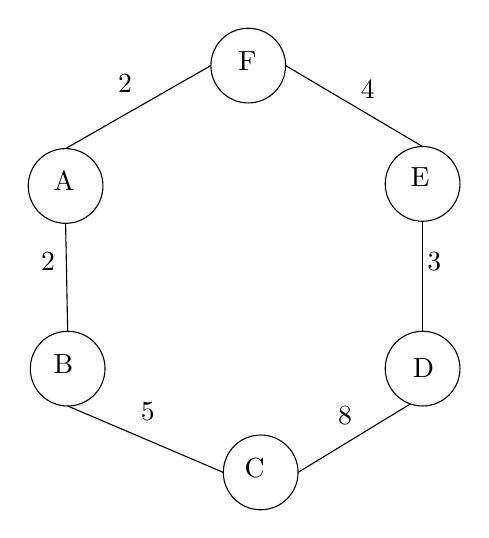
\begin{tikzpicture}[x=0.75pt,y=0.75pt,yscale=-1,xscale=1]
		%uncomment if require: \path (0,300); %set diagram left start at 0, and has height of 300
		
		%Shape: Circle [id:dp74630576412552] 
		\draw   (303,48) .. controls (303,38.06) and (311.06,30) .. (321,30) .. controls (330.94,30) and (339,38.06) .. (339,48) .. controls (339,57.94) and (330.94,66) .. (321,66) .. controls (311.06,66) and (303,57.94) .. (303,48) -- cycle ;
		%Shape: Circle [id:dp6948502936863147] 
		\draw   (309,244) .. controls (309,234.06) and (317.06,226) .. (327,226) .. controls (336.94,226) and (345,234.06) .. (345,244) .. controls (345,253.94) and (336.94,262) .. (327,262) .. controls (317.06,262) and (309,253.94) .. (309,244) -- cycle ;
		%Shape: Circle [id:dp411524330774953] 
		\draw   (387,105) .. controls (387,95.06) and (395.06,87) .. (405,87) .. controls (414.94,87) and (423,95.06) .. (423,105) .. controls (423,114.94) and (414.94,123) .. (405,123) .. controls (395.06,123) and (387,114.94) .. (387,105) -- cycle ;
		%Shape: Circle [id:dp9061935864250484] 
		\draw   (387,194) .. controls (387,184.06) and (395.06,176) .. (405,176) .. controls (414.94,176) and (423,184.06) .. (423,194) .. controls (423,203.94) and (414.94,212) .. (405,212) .. controls (395.06,212) and (387,203.94) .. (387,194) -- cycle ;
		%Shape: Circle [id:dp8935414105757558] 
		\draw   (215,106) .. controls (215,96.06) and (223.06,88) .. (233,88) .. controls (242.94,88) and (251,96.06) .. (251,106) .. controls (251,115.94) and (242.94,124) .. (233,124) .. controls (223.06,124) and (215,115.94) .. (215,106) -- cycle ;
		%Shape: Circle [id:dp6332889169878556] 
		\draw   (216,194) .. controls (216,184.06) and (224.06,176) .. (234,176) .. controls (243.94,176) and (252,184.06) .. (252,194) .. controls (252,203.94) and (243.94,212) .. (234,212) .. controls (224.06,212) and (216,203.94) .. (216,194) -- cycle ;
		%Straight Lines [id:da44971170608866995] 
		\draw    (233,88) -- (303,48) ;
		%Straight Lines [id:da5363060221925924] 
		\draw    (405,87) -- (339,48) ;
		%Straight Lines [id:da05648797244313897] 
		\draw    (233,124) -- (234,176) ;
		%Straight Lines [id:da4867338445672943] 
		\draw    (309,244) -- (234,212) ;
		%Straight Lines [id:da4987941822532661] 
		\draw    (345,244) -- (399.13,211) ;
		%Straight Lines [id:da7879798993739897] 
		\draw    (405,176) -- (405,123) ;
		
		% Text Node
		\draw (257,51) node [anchor=north west][inner sep=0.75pt]   [align=left] {2};
		% Text Node
		\draw (374,54) node [anchor=north west][inner sep=0.75pt]   [align=left] {4};
		% Text Node
		\draw (406,137) node [anchor=north west][inner sep=0.75pt]   [align=left] {3};
		% Text Node
		\draw (363,211) node [anchor=north west][inner sep=0.75pt]   [align=left] {8};
		% Text Node
		\draw (268,209) node [anchor=north west][inner sep=0.75pt]   [align=left] {5};
		% Text Node
		\draw (220,137) node [anchor=north west][inner sep=0.75pt]   [align=left] {2};
		% Text Node
		\draw (315,40) node [anchor=north west][inner sep=0.75pt]   [align=left] {F};
		% Text Node
		\draw (398,96) node [anchor=north west][inner sep=0.75pt]   [align=left] {E};
		% Text Node
		\draw (399,188) node [anchor=north west][inner sep=0.75pt]   [align=left] {D};
		% Text Node
		\draw (318,236) node [anchor=north west][inner sep=0.75pt]   [align=left] {C};
		% Text Node
		\draw (226,186) node [anchor=north west][inner sep=0.75pt]   [align=left] {B};
		% Text Node
		\draw (226,98) node [anchor=north west][inner sep=0.75pt]   [align=left] {A};
		
		
		\end{tikzpicture}
				
		\caption{Network}
		\label{2}
		
	\end{figure}
	        
	
	

	


	
	
\end{document}
